\documentclass{standalone}
\usepackage{amsmath}
\usepackage{amssymb}
\usepackage{listings}
\usepackage{tikz}
\usepackage{xcolor}

\usetikzlibrary{calc}
\usetikzlibrary{backgrounds}
\definecolor{base3}{HTML}{fdf6e3}
\definecolor{blue}{HTML}{268bd2}
\definecolor{green}{HTML}{859900}
\definecolor{magenta}{HTML}{d33682}

\begin{document}

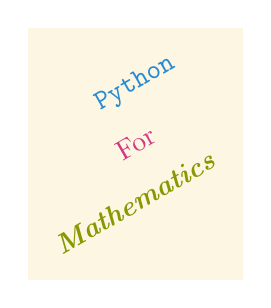
\begin{tikzpicture}[background rectangle/.style={fill=base3}, show background rectangle]
    \node (python) [rotate=30, color=blue] at (0, 0) {\texttt{Python}};
    \node (for) [rotate=30, color=magenta] at ($(python) + (0, -.75)$) {For};
    \node (mathematics) [rotate=30, color=green] at ($(for) + (0, -.75)$) {\textit{\textbf{Mathematics}}};
\end{tikzpicture}
\end{document} 
